
\iffalse
\begin{definition}[Continuous Time]
The continuous time limit is a sequence of games indexed by
$j=0,1,\ldots$. Suppose the stopping time for all games is equal to
$T$.
Let $s_i^j$ be the step size associated with the
$i'th$ iteration of game $j$. Then $s_i^j$ are supposed to have the
following properties:
\begin{itemize}
\item Let $s^j = \max_i s_i^j$, then $\lim_{j \to \infty} s^j = 0$
  \item for any $j$, $\sum_i (s_i^j)^2 = T$
\end{itemize}
  \end{definition}

\section{Old Stuff}





\section{Variable time steps}
The second order bounds of~\cite{cesa2007improved} show that, in some
contexts, the time parameter $t$ can be replaced by a variance-type
parameter $\V_T= \sum_{i=1}^T \var_i$. This corresponds to a
significant tightening of the bound. For example if instead of $l_j^i
\in [-\epsilon,+\epsilon]$, then $\V_T = T\epsilon^2$, and if we set
$T=\epsilon^{-2}$ we get n upper bound on the regret that does not
depend on $T$. The idea is to replace $T$ with $V_T$ in the definition
of the upper and lower potentials. Which is what we do in
Section\ref{sec:discrete}.

In that variant of the potential game the adversary chooses the
``real-time'' step at each iteration. Surprisingly, it turns out that
the adversary's preference is to make the time steps as small as
possible (but not zero). Combining the random walk strategy with the
infinitesimal time step, we arrive at a strategy that is define by
Brownian motion, or a Wiener process. Even more surprisingly, the
strategy of the learning at this limit corresponds to the same
Brownian motion. In other words, we have a min-max characterization of
DTOL.

\paragraph*{The rest of the paper is organized as follows}
In Section~\ref{sec:preliminaries} we provide some basic definitions.
In Section~\ref{sec:integer} we describe the potential game in the standard
integer time case and prove some upper and lower bounds for this
case. In Section~\ref{sec:discrete} we define a the discrete time
game, where time advances are real valued and finite. The core of our
argument, which is based on the theory of ``divided-differences''
appears in Section~\ref{sec:smallsteps}. In
Section~\ref{sec:continuous} we define the continuous time limit of
the game. In Section~\ref{sec:self-consistent} we show that optimal
any-time potential functions correspond to the solution of the
kolmogorov Backwards differential equation, and show the Exponential weights and
NormalHedge are solutions for that Equation. Finally, in
Section~\ref{sec:NormalHedge}
we argue that NormalHedge is the best possible potential function.

  \fi

  \iffalse
\subsubsection*{Our Contributions}
\begin{itemize}
\item We characterize the min/max strategies for 
  potential functions that have strictly positive derivatives up to
  order four.
\item We show that the optimal adversarial strategy for all of
  these potential functions is a strategy corresponding to
  Brownian motion.
\item We show that $V_T$ replaces $T$ for any of these games.
\item  We show that all potential functions that satisfy a particular
  partial differential equations yield min/max solutions to the
  potential game.
\item We show that both the exponential weights algorithm and
  NormalHedge are solutions to the PDE.
  \item We show that NormalHedge provides the best possible regret bounds.
\end{itemize}

In this paper we extend and refine the analysis of the potential
function to
provide a min/max analysis for a large set of potential functions. We
then show that NormalHedge is, in a strong sense the best of those
potential functions.

Our analysis is based on three ideas that are listed below.
\begin{itemize}
    \item {\bf Potential games:} We focus on the potential function, rather than on the problem of minimizing regret. In other words, we define a new game, in which the goal of the learner is to minimize  the final average potential.
    \item {\bf Experts as a probability space:} Instead of restricting the game to $N$ strategies, we allow the set of strategies to be an arbitrary probability space. This allows the adversary the following simple but powerful strategy.  At each iteration $i$ the adversary splits each one of the strategies into two equal parts, once part incurs loss $-1$ and the other loss $+1$. In other words, at iteration $i$ there are $2^i$ strategies, each corresponding to a sequence in $\{-1,+1\}^i$. It is intuitively clear that the instantaneous loss of the learner is always zero, regardless of it's choice of $P$.
    \item {\bf Reducing the time step and continuous time:} Regret bounds of the form $C\sqrt{T \ln N}$ are tight for the case in which the adversary assigns losses of $\pm 1$ with equal probabilities.
    Suppose however, that the adversary produces the exact same sequence of losses, but divides the range of each loss by 2. In this case the losses and the regrets will all be divided by two, but the bound will remain the same! This suggest that defining $T$ as the number of iterations in the game leaves some slack. To remedy this situation we let time take on real values such that $t_{i+1}-t_i \leq 1$. At the same time we 
    allow the adversary to declare, before each iteration, the range $[-s_i,+s_i]$ for the losses, in which case the following time would be 
    $t_{i+1}=t_i +s_i^2$. Surprisingly, we find out that for a large set of potential functions, the preference of the adversary is to make $s_i$ as small as possible, making iterative game into a continuous time game and the adversarial strategy to be Brownian motion.
\end{itemize}

  \subsection{A learner strategy with a variance-dependent bound}

  As shown in Lemma~\ref{lemma:adversary-prefers-extremes}, the
  adversary always prefers mixed strategies that assign zero
  probability for all steps other than $\pm 1$. Suppose, however, that
  the adversary is not worst-case optimal and chooses steps whose
  length is less than one. The following lemma gives a slightly
  different strategy for the learner, which guarantees a tighter bound
  for this case.

  \begin{lemma} \label{lemma:second-order-bound}
      The learner strategy:
      \begin{equation} \label{eqn:learner-strat-2}
      \learnerM^2(i-1,\R) =  \frac{1}{Z}
      \left. \frac{\partial}{\partial r} \right|_{r=\R} \pot(i,r)
      \end{equation}
      Where $Z$ is a normalization factor
      $$Z = \E{\R \sim \state(i)}{\left. \frac{\partial}{\partial r} \right|_{r=\R} \pot(i,r)}$$
      guarantees the following upper potential against any adversarial
      strategy $\adversM$
      \begin{equation} \label{eqn:value-iteration-upper}
        \upperpot(i-1, \R) = \pot(i,\R) + b(i,\R) \E{l \sim \adversM(i,\R)}{l^2}
      \end{equation}
      where $b(i,\R) = \pot(i,\R+2) -\pot(i,\R) - 2 \left. \frac{\partial}{\partial r} \right|_{r=\R} \pot(i,r)$
   \end{lemma}

   \proof
   To Do
   \qed
   
We compare the bound for $\learnerM^2$ to the bound for $\learnerM^1$
given in Lemma~\ref{lemma:first-order-bound}. We find that when the 
adversary is optimal: $\E{l \sim \adversM(t,\R)}{l^2}=1$ then the
bound for $\learnerM^1$ is better than the bound for $\learnerM^2$, on the
other hand, when $\E{l \sim \adversM(t,\R)}{l^2}$ is close to zero,
$\learnerM^2$ is better than $\learnerM^1$.  

\fi

\iffalse
We start with motivation for using time that is indexed by real
values rather than the natural numbers. We distinguish between two
notions of time. The first notion of time is a counter that
counts the iterations of the game, we will call this counter the {\em
  iteration counter } and denote it by $i=0,1,\ldots$. The second,
more interesting notion of time is the time that appears in the regret
bounds, we denote this time by $t_i$ where $i$ is the iteration
number. We restrict the time increments $\Delta t_i =t_i-t_{i-1}$ to
the range $0\leq \Delta t_i \leq 1$.  The magnitude of $\deltat_i$
corresponds to the {\em hardness} of iteration $i$. $\deltat_i=0$
corresponds to the case where the losses of all of the strategies are
equal to a common value $-1 \leq a \leq 1$. In this case the aggregate
loss $\ell=a$, the state does not change:
$\state(i-1)=\state(i)$, $\Delta t_i=0$ and the instantanous regret is zero. On the
other hand $\Delta t_i=1$ corresponds to the adversarial strategy
$\adversM^{1/2}(t-1,R)$ (Eqn.~\ref{eqn:adv-strat}) which maximizes the
instantanous regret.

We introduce an additional step to the integer game. Before the
learner makes it's choice, the 
adversary chooses a real number $0 \leq s_i \leq 1$, by doing so, the
adversary commits that all of the instantanous expert lossesat that
step be in the range $[-s_i,s_i]$. The time step is defined to be $\deltat_i =
s_i^2$.

First, note that the adversary in this game is at least as powerful as
the adversary in the integer game. This is because the adversary can
always choose $s_i=1$, effectively reducing the game to the integer
game.

Next, we justify the choice $\deltat_i = s_i^2$. Our argument is that
any significantly different choice would give the game to one side or
the other.  Suppose that $s_i = 1/k$ on all $m_k$ iterations of the game. In
other words, this is a rescaling of the integer game. Consider the
adversarial strategy. The distribution (state) after $m_k$ iterations is the
binomial distribution. with mean zero and variance $m_k \frac{1}{k^2}$
if $m_k \gg \frac{1}{k^2}$ then the variance at the end of the game
goes to infinity.

By allowing $\Delta t_i$ to vary from iteration to iteration
we get a more refined quantification of the regret and, as we show
below, min/max optimality.

To find the relationship between loss magnitude and time increments 
we compare two adversarial strategies.  The first strategy, discussed above,
generates losses $\pm 1$ with equal probability, we deonte this
strategy by $\adversM^{1/2}_{\pm 1}$. The other strategy, denoted
$\adversM^{1/2}_{\pm 1/k}$, generates losses of $\pm 1/k$ with equal
probabilities.

From the adversarial point of view $\adversM^{1/2}_{\pm 1/k}$ is worse
than $\adversM^{1/2}_{\pm 1}$. So it should correspond to a smaller
time increment. But how much smaller? Suppose we start with the
initial state $\state(0)$ which is a delta functions at $\R=0$.  One
iteration of $\adversM^{1/2}_{\pm 1}$ results in a distribution
$\pm 1$ w.p, $(1/2,1/2)$, which has mean $0$ and variance $1$.
Suppose we associate $\Delta t =1/j$ with a single step of
$\adversM^{1/2}_{\pm 1/k}$.  Equivalently, we associate $j$ iterations
of $\adversM^{1/2}_{\pm 1/k}$ with $t=1$.  How should we set $j$? the
distribution generated by $j$ steps is a binomial distribution
supported on $j+1$ points, so there is no hope of making the two
distributions identical. However, as it turns out, it is enough to
equalize the mean and the variance of the two distributions. The mean
of $\adversM^{1/2}_{\pm 1/k}$ is zero for any $k$. As for the
variances, a single iteration of $\adversM^{1/2}_{\pm 1}$ is 1 and a
single iteration of $\adversM^{1/2}_{\pm 1/k}$ is $1/k^2$. It follows
that the variance after $j$ iterations of $\adversM^{1/2}_{\pm 1/k}$
$j/k^2$. Equating this variance with that of a single step of
$\adversM^{1/2}_{\pm 1}$ we get $j=k^2$ and $\Delta t= 1/k^2$.

Note a curious behaviour of the {\em range} of $\R$ as $k \to \infty$
the number of steps increases like $k^2$ while the size of each step
is $1/k$. This means that the range of $\R$ is $[-k,k]$, which becomes
converges to $(-\infty, + \infty)$ when $k \to \infty$. On the other
hand, the variance increases like $t$.

Next lets consider effect of reducing the step size on a {\em biased}
strategy $\adversM^{1/2+\gamma}_{\pm 1}$ as defined in
Eqn~(\ref{eqn:adv-strat-p}) for some
$0\leq \gamma \leq 1/2$.  We now figure out what  $\gamma'$ should be
so that the distribution generated by $k^2$ iterations of $\adversM^{1/2+\gamma'}_{\pm 1/k}$ has the
same mean as a single iteration of $\adversM^{1/2+\gamma}_{\pm
  1}$. The mean of a single iteration of
$\adversM^{1/2+\gamma}_{\pm 1}$ is $2\gamma$ while the mean of a
single iteration of $\adversM^{1/2+\gamma'}_{\pm 1/k}$ is
$2\gamma'/k$. Therefor to keep the means equal we need to set
$2\gamma'/k = 2\gamma$ or $\gamma' = \gamma/k$.


Note that as $k \to \infty$, $\gamma' \to 0$. This observation
motivates scaling the bound on $\ell(t)$ like $c s_i^2$ (see the
description of the game below.)

This leads to the following formulation of a continuous time game.
The game is a generalization of the integer time game in that by
always choosing $s_i=1$ the adversary forces the integer time game.

In this game we use $i=1,2,3,\ldots$ as the iteration index. We use
$t_i$ to indicate a sequence of real-valued time points. $t_0=0$ and
we assume there exists a finite $n$ such that $t_n = T$.

We will later give some particular potential functions for which no
a-priori knowledge of the termination condition is needed. The
associated bounds will hold for any iteration of the game.

\iffalse
Consider the states at two consecutive iterations $\state(i-1),\state(i)$.
Suppose that $\pot(i,\R)$, the value function for iteration $i$ is fixed.
We say that $\lowerpot(i-1,\R)$ is a lower bound on the value at iteration
$i-1$ if there is exists an adversarial strategy $\adversM^*$ such that
for any strategy of the learner $\learnerM$, 
$$ \E{\R \sim \state(i-1)}{\lowerpot(i-1)} \leq \E{\R \sim \state(i)}{\pot(i)}$$
Similarly, $\upperpot(i-1,\R)$ is an upper potential if there exists a
learner strategy $\learnerM^*$ such that for any adversarial strategy
$\adversM$,
$$ \E{\R \sim \state(i-1)}{\upperpot(i-1)} \geq \E{\R \sim \state(i)}{\pot(i)}$$



  We find that the lower bound corredponds to an unbiased random
  walk with step size $\pm 1$. The upper bound also corresponds to a an
  unbiasd random walk with step size $\pm(1+c)$. The natural setting
  in the natural game is $c=1$, which means that there is a
  significant difference between the upper and lower bounds. As we
  show in the next section, this gap converges to zero in the
  continuous time setting, and the upper and lower bounds match,
  making the strategies for both sides min-max optimal. 

  Note also that the adversarial strategy the aggregate loss
  $\ell(t)$ is always zero, regardless of the strategy of the
  learner, and state progression is independent of the
  learner's choices.
\fi
  \begin{figure}[t]
%\vskip -0.2in
\begin{center}

 \centerline{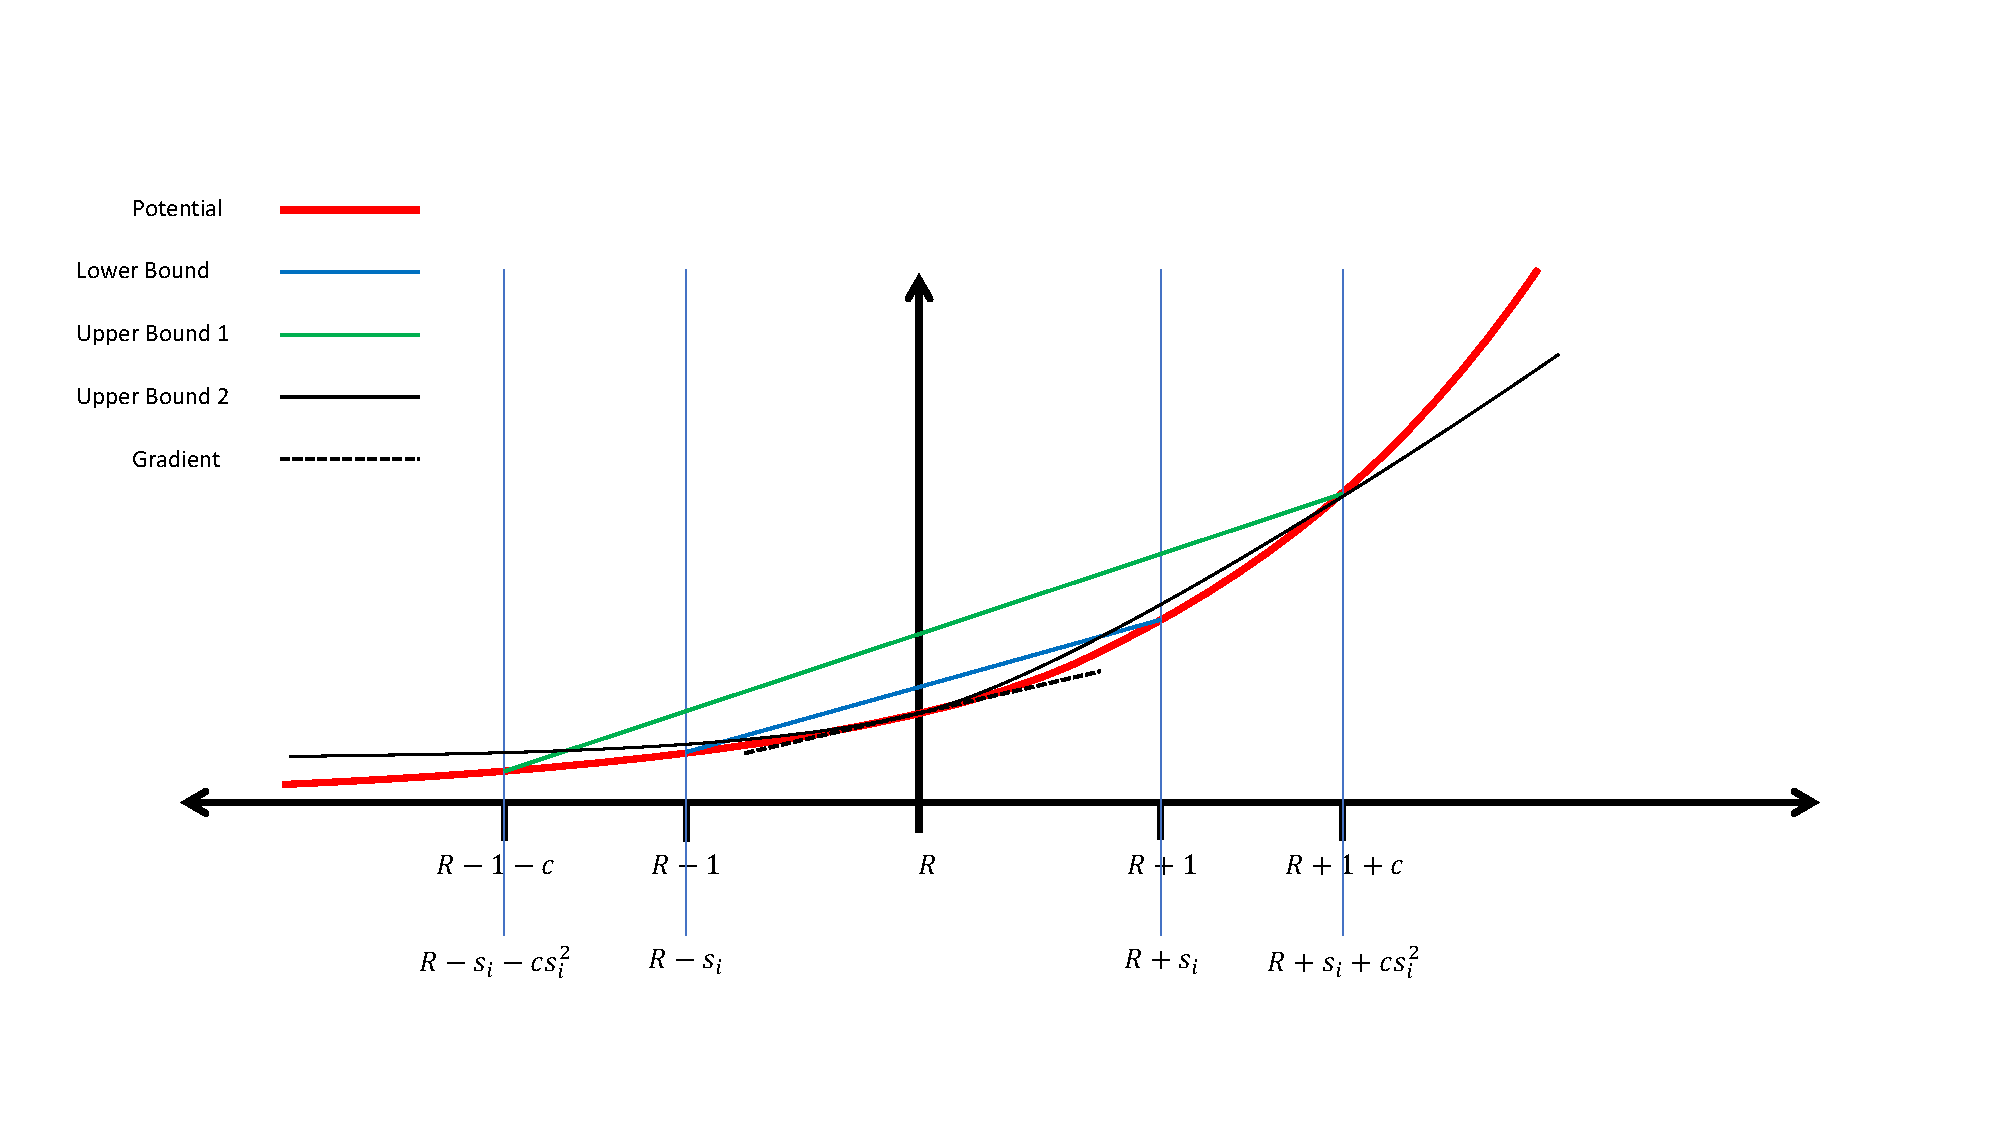
\includegraphics[width=\textwidth]{figures/convexPot.pdf}}
\caption{This figure depicts the relationship between the different
  upper and lower bounds used in the analysis. To aid understanding we
  describe the elements of the figure twice: once for the integer
  game, and once for the continuous time game. \newline
  {\bf Integer time game:} let
  the current iteration be $i$ and let the current regret be $\R$. Let
  $r$ be the regret at iteration $i+1$, we have that $\R-2 \leq r
  \leq \R+2$. The potential at iteration $i+1$ is $\pot(i+1,r)$ (the red curve). The lower bound
  (blue line) corresponds to the adversarial strategy:
  $\adversM^{1/2}(i,\R)$. The first-order learner strategy:
  $\learnerM^1(i,\R)$ corresponds to the green line. The second-order
  learner strategy:  $\learnerM^2(i,\R)$ corresponds to the black
  curve.\newline
{\bf Continuous time game:} let
  the current iteration be $i$, the current time be $t_i$ and the
  current regret be $\R$. Let $0<s_i\leq 1$ be the step size chosen by the
  adversary, so that the next time is $t_{i+1} = t_i+s_i^2$. Let $r$
  be the regret at iteration
  $i+1$, we have that $\R-s_i-c s_i^2 \leq r \leq \R+s_i+c s_i^2$.
  The potential at iteration $i+1$ is $\pot(t_{i+1},r)$ (the red
  curve).  The lower bound (blue line) corresponds to the adversarial
  strategy: $\adversM^{1/2}_{\pm s_i}(t_i,\R)$. The first-order learner strategy:
  $\learnerM^{1c}(t_i,\R)$ corresponds to the green line. The second-order
  learner strategy: $\learnerM^{2c}(i,\R)$ corresponds to the black
  curve.   Observe that when $s_i \to 0$ the ratio $\frac{s_i}{s_i+c
    s_i^2}$ converges to 1, and the upper and gap between the green
  and blue lines converges to zero.\\
\rule[1ex]{6.5in}{0.5pt}}
\label{fig:ConvexPot}
\end{center}
\vskip -0.4in
\end{figure} 


%%%%%%%%%%%%

number of iterations by the
total variance. 
The time on iteration $i+1$ is $t_{i+1}=t_i+s_i^2$. To motivate this
update consider the natural extension of the adversarial and learner
strategies~(\ref{eqn:adv-strat-p},\ref{eqn:learner-strat-1})
for an arbitrary $0<s_i\leq 1$.

The adversarial strategy is 
\begin{equation} \label{eqn:adv-strat-s}
  \adversM^I(i-1,\R) =
  \begin{cases}
    +s_i & \mbox{ w.p. } \frac{1}{2}\\
    -s_i & \mbox{ w.p. } \frac{1}{2}\\
  \end{cases}
\end{equation}

and the learner strategy is
\begin{equation} \label{eqn:learner-strat-s}
\learnerM^I(i-1,\R) = \frac{1}{Z} \frac{\pot(i,\R+2s_i) - \pot(i,\R-2s_i)}{2}
\end{equation}
Where $Z$ is a normalization factor.



Following the same line of argument as in the proof of
Theorem~(\ref{thm:IntegerGameBounds}), and specializing for
$i=0,\R_0=0$ we get the bounds

  \begin{itemize}
  \item
    The adversarial strategy~(\ref{eqn:adv-strat-s}) starting from
    $\state(i,\R_0)$. Guarantees a final potential 
     
    $$\score(T) \geq \E{\R \sim B(\langle s_0,\ldots,s_{T-1}\rangle)}{\pot(T,\R)}$$
  \item
    There learner strategy~(\ref{eqn:learner-strat-s}) guarantees
    $$\score(T) \geq \E{\R \sim B(\langle 2s_0,\ldots,2s_{T-1}\rangle)}{\pot(T,\R)}$$
  \end{itemize}

Where for any sequence of $T$ non-negative numbers
$a_0,\ldots,a_{T-1}$
we denote by $B(\langle a_0,\ldots,a_{T-1}\rangle)$ the distribution of
the sum of $T$ i.i.d. random variables
$$X_i =   \begin{cases}
    +a_i & \mbox{ w.p. } \frac{1}{2}\\
    -a_i & \mbox{ w.p. } \frac{1}{2}\\
  \end{cases}
$$
It is easy to verify that  $B(\langle a_0,\ldots,a_{T-1}\rangle)$ is a
symmetric distribution with mean zero and variance $\sum_{i=0}^{T-1}
a_i^2$. 

\section{More on scaling}

-------
Suppose we set $p=1/2$ and $s=1$ or $s=1/2$.
Following the proof of
theorem~(\ref{thm:IntegerGameBounds}) it is not hard to show that


For some intuition consider repeating for $N$ iterations either  
$\adversM^s(i-1,\R,1,1/2)$ and $\adversM^s(i-1,\R,1/2,1/2)$.
From Theorem~({thm:IntegerGameBounds}) 


that these strategies
guarantee lower potentials 

It is not hard
to show that the distribution of the regret $\R$  after $N$ iterations
is $B(N,1)$ in the first case and $B(N,1/2)$ in the second
case. 



using the total variance instead of
the number of steps. We define a generalization of the adversarial


We conclude that it is the total variance, and not the number of
iterations, that determines the final score. We define the total
variance at iteration $i$ to be the {\em time} at iteration $i$ which
we denote by $t_i$. The uprate rule for the time is $t_{i+1}=t_i+s_i^2$. 
As expected, in the integer time game $s_i=1$ which
implies that $t_i = i$.

Without additional restrictions, this game advantages the
adversary. We now sketch an adversarial strategy by which the
adversary can force the final score to be arbitrarily large.
The adversarial strategy is an uncentered variant of
to $\adversM^s$ (Equation~(\ref{eqn:adv-strat-s}))
\begin{equation} \label{eqn:adv-strat-k}
  \adversM^k(i,\R) =
  \begin{cases}
    0 & \mbox{ w.p. } \frac{1}{2}\\
    -1/k  & \mbox{ w.p. } \frac{1}{2}\\
  \end{cases}
\end{equation}

We set the number of iterations $N_k=4k^2$ so that the total variance
at the end is $N_k V_1= \frac{4k^2}{4k^2}=1$. The loss of the learner
on each iteration is $1/2k$ and therefor the total loss is $N_k/2k =
\frac{4k^2}{2k} = 2k$.


In this case $s_i=1/k$, we set the number of iterations to $N=k^2$ so
that the final time (or total variance) is $1$. Note that the expected
total loss (total learner loss) is $N (3/4-1/4)/k = k/2$. In other words, as $k \to \infty$
the total loss of the learner also goes to infinity. We avoid this
case by requiring that the single iteration learner loss is at most
$s_i^2$.
% ~\footnote{We conjecture that removing this requirements
%   implies the existance of adversarial strategies that guarantee that
%   the final score is arbitrarily high, regardless of the learner's
%   strategy. Demonstrating such a strategy is an open problem.}


\fi

\iffalse
\begin{lemma} \label{lemma:adversary-prefers-extremes}
 Suppose $\lowerpot(i,\R)$ is strictly convex with respect to  $\R$.
Let ${\cal Q}(i-1,\R,\Bias)$ be the set of adversarial strategies 
$\adversM(i-1,\R)$ that have bias
$\Bias=\Bias(i-1,\R)= \E{y \sim \adversM(i-1,\R)}{y}$ then the
strategy in ${\cal Q}(i-1,\R,\Bias)$ that is best for the adversary is

\begin{equation} \label{eqn:value-iteration-lower-recursion}
  \lowerpot(i-1, \R) = p \lowerpot(i,\R+1) + (1-p)\lowerpot(i,\R-1)
\end{equation}
which is strictly higher than $\lowerpot(i-1,\R)$ for any other
distribution in ${\cal Q}(i-1,\R,\Bias)$. In addition,
$\lowerpot(i-1, \R)$ is strictly convex.
\end{lemma}


%%%%%%%%%%%%%%%%%%%%%%%%%%%%%%%%%%%%%
\item Suppose we fix the strategies for iterations $i+1,\ldots
  T-1$, and the value of the average loss $\ell(i)$, Then the
  strategies for both the learner and the adversary can be optimized
  for each value of $\R$ independently. In other words, there are no
  interactions (other than through $\ell(i)$) between changes


\fi

\iffalse
$\epsilon>0$ such that
for any $v>0$ there exists $|h_v(x)| < v$ such that 
$|\E{x \sim \state}{h_v(x) f'(x)}|>\epsilon$. Define $h'_v =
\frac{h_v}{v}$. Clearly $|h'_v(x)|<1$ and we have that
$$|\E{x \sim \state}{h'_v(x) f'(x)}|>\frac{\epsilon}{v}$$

Define the positive parts of $h_v$ to be $h_v^+(x) = \max(0,h'_v(x))$
and $h_v^-(x) = \max(0,-h'_v(x))$. As $f'(x)>0$ we that either
\[
  \E{x \sim \state}{h^+_v(x) f'(x)}>\frac{\epsilon}{v}
\]
or 
\[
  \E{x \sim \state}{h^-_v(x) f'(x)}>\frac{\epsilon}{v}
\]
Wlog assume the first. As $f \in \SP{2}$, we have that $f(x+1) \geq f'(x)$. Therefore
 $\E{x \sim \state}{f(x+1)|h_v^(x)>0)}=\infty$. As $f(x)>0$ for all $x$ we
 find that $\E{x \sim \state}{f(x)}=\infty$ which contradicts the
 Lemma's assumption.
\qed
\fi
